\documentclass{article}

\usepackage[pdftex]{graphicx}

\usepackage{svg}
\usepackage{listings}
\usepackage{color}
\usepackage{times}
\usepackage{amsfonts}
\usepackage{draftwatermark}
\SetWatermarkText{DRAFT}
\SetWatermarkScale{1}
\SetWatermarkLightness{0.95}

\lstset{
float, 
mathescape=true, 
texcl=true,
basicstyle=\footnotesize\ttfamily,
columns=fixed,
numbers=none,%left,
stepnumber=1,
captionpos=b,
showstringspaces=true,
language=C++,
keywordstyle=\color[rgb]{0.0, 0.0, 0.8},
stringstyle=\color[rgb]{0.5, 0.0, 0.5},
tabsize=4,
commentstyle=\color[rgb]{0.133,0.545,0.133}\textit,
morekeywords={ },
frame=single,
}

\begin{document}

\title{Dynamic Trees}
\author{Erin Catto\\Blizzard Entertainment}
\maketitle

\begin{abstract}
\small
This document presents techniques for using dynamic AABB trees in games to handle incremental updates to the tree structure. Tree insertions are optimized using the Surface Area Heuristic combined with sub-tree rotations. The tree is also optimized in an iterative fashion using rotations and shuffle operations.
\end{abstract}

\section{Introduction}

Physics engines for games usually have a \emph{broad-phase} to accelerate ray casts, shape casts, and overlap tests. Typically there are many independently moving objects along with that static environment that need to be considered. Furthermore, steaming environments need to load and unload both static and dynamic objects.

For simple games, a brute force approach with an array of axis-aligned bounding boxes (AABBs) can suffice. Once there are more than 20 or so objects, a better acceleration structure can improve performance. 

There are other data structures that work for dynamic environments. The two main data structures used in modern physics engines are the sweep-and-prune sparse grid and dynamic AABB trees. Sweep-and-prune data structure has recently fallen out of favor due to poor scaling for long ray casts in large worlds.

This leaves the dynamic AABB tree as the favorite among many of the physics engines in active development. There are a number of techniques that can be applied to an AABB tree to make it suitable for dynamic worlds. These will be covered in the following sections.

\cite{Bittner2013}

\section{AABB Trees}
Figure~\ref{fig:loose} shows several geometric objects that may exist in a game world. Gameplay code may wish to query this world to make decisions. Queries are usually ray casts and overlap tests. For example in a shooting game a ray cast can represent the projectile. Area effects may use an overlap test to determine what objects are present in a region of space, typically an AABB or spherical region.

\begin{figure}
	\begin{center}
		\includesvg[width=0.6\textwidth]{LooseObjects}
	\end{center}
	\caption{Objects in a game world}
	\label{fig:loose}
\end{figure}

\begin{figure}
	\begin{center}
		\includesvg[width=0.6\textwidth]{LooseRayCast}
	\end{center}
	\caption{Ray-cast against game world}
	\label{fig:raycast}
\end{figure}

\begin{lstlisting}[caption={Brute-force ray-casting}, label={lst:brute_ray}, float]
bool BruteForceRayCast(Vec3 rayStart, Vec3 rayEnd)
{
	for (int i = 0; i < objectCount; ++i)
	{
		bool hit = objects[i].RayCast(rayStart, rayEnd);
		if (hit)
		{
			return true;
		}
	}
	return false
}
\end{lstlisting}

\begin{figure}
	\begin{center}
		\includesvg[width=0.6\textwidth]{LooseOverlap}
	\end{center}
	\caption{Overlap test in game world}
	\label{fig:overlap}
\end{figure}

\begin{lstlisting}[caption={Brute-force overlap test}, label={lst:brute_overlap}, float]
Vector<int> BruteForceOverlapTest(AABB queryAABB)
{
	Vector<int> results;
	for (int i = 0; i < objectCount; ++i)
	{
		bool overlap = objects[i].OverlapTest(queryAABB);
		if (overlap)
		{
			results.PushBack(i);
		}
	}
	return results;
}
\end{lstlisting}

Brute-force testing becomes slow in large worlds. Ray-cast and overlap queries can be made faster by organizing the geometric objects into a bounding volume hierarchy (BVH). A BVH groups objects that are spatially close inside an encasing geometric object (bounding volume). This is setup recursively so that BVH groups are also grouped together until at the root of the tree there is a single bounding volume that encases all objects.

AABB trees are a popular BVH due to their simplicity and effectiveness. Each node of the tree has an associated AABB that encases the child nodes. A node can be an internal node or a leaf node. The leaf nodes contain a reference to the geometric objects. Listing~\ref{lst:node} shows a basic tree node. It has the AABB, a flag to indicate if it is a leaf node, a pointer to the geometric object (when it is a leaf node), indices of the child nodes and parent node. The geometric object pointer is null when isLeaf is false. The child indices are -1 when the node is a leaf. The parent index is -1 when the node is the root node of the tree.
\begin{lstlisting}[caption={AABB tree node}, label={lst:node}, float]
struct AABBNode
{
	AABB aabb;
	bool isLeaf;
	int objectIndex;
	int child1;
	int child2;
	int parent;
}
\end{lstlisting}

The AABB tree can be represented as an array of nodes. The convention is that the first node in the array is the root. The indices in the nodes refer to other nodes in the node array.

\begin{lstlisting}[caption={AABB tree}, label={lst:tree}, float]
struct AABBTree
{
	AABBNode* nodes;
	int count;
}
\end{lstlisting}

Figure~\ref{fig:overlay} shows an AABB tree overlayed onto the game world. The colored dashed boxes represent internal nodes in the tree. Different colors represent different levels in the tree. Figure~\ref{fig:example_tree} shows the associated binary tree. Each leaf node is square and represents the geometric objects in the game world. Unlike a binary search tree, the order of the leaf nodes is not vital.
\begin{figure}
	\begin{center}
		\includesvg[pretex=\large, width=0.6\textwidth]{TreeOverlay}
	\end{center}
	\caption{AABB tree overlayed onto game world}
	\label{fig:overlay}
\end{figure}

\begin{figure}
	\begin{center}
		\includesvg[pretex=\large, width=\textwidth]{ExampleBinaryTree}
	\end{center}
	\caption{Example binary tree}
	\label{fig:example_tree}
\end{figure}

The structural requirements for an AABB are as follows:
\begin{itemize}
	\item Every internal node has exactly two children
	\item Every leaf node has no children
	\item Every internal node has an AABB that is the union of the child AABBs
\end{itemize}

A ray-cast and overlap algorithms are built using this structure. Standard tree traveral techniques are used and a stack data structure is used instead of functional recursion. Listings~\ref{lst:tree_ray} and \ref{lst:tree_overlap} give basic examples of tree traversal. They both use a stack data structure and rely on external functions for object level ray-casts and overlap tests. Some refinements are left out, such as ray clipping, AABB tests, and detailed results.

\begin{lstlisting}[caption={Tree ray-cast}, label={lst:tree_ray}, float]
bool TreeRayCast(Vec3 rayStart, Vec3 rayEnd)
{
	Stack<int> s;
	s.Push(0);
	while (stack.IsEmpty() == false)
	{
		int index = s.Pop();
		if (nodes[index].AABB.Overlap(rayStart, rayEnd) == false)
		{
			continue;
		}

		if (nodes[index].isLeaf)
		{
			int objectIndex = nodes[index].objectIndex;
			if (objects[objectIndex].RayCast(rayStart, rayEnd))
			{
				return true;
			}
		}
		else
		{
			s.Push(nodes[index].child1);
			s.Push(nodes[index].child2);
		}
	}

	return false;
}
\end{lstlisting}

\begin{lstlisting}[caption={Tree overlap test}, label={lst:tree_overlap}, float]
Vector<int> TreeOverlapTest(AABB queryAABB)
{
	Vector<int> results;
	Stack<int> s;
	s.Push(0);
	while (stack.IsEmpty() == false)
	{
		int index = s.Pop();
		int objectIndex = nodes[index].objectIndex;
		if (objects[objectIndex].OverlapTest(queryAABB) == false)
		{
			continue;
		}

		if (nodes[index].isLeaf)
		{
			results.PushBack(objectIndex);
		}
		else
		{
			s.Push(nodes[index].child1);
			s.Push(nodes[index].child2);
		}
	}

	return false;
}
\end{lstlisting}

\section{Surface Area Heuristic}
The AABB tree shown in Figures~\ref{fig:overlay} and \ref{fig:example_tree} is just one possible tree out of many. This gives rise to a couple questions:
\begin{enumerate}
	\item What is the optimal tree?
	\item How can an optimal tree be generated automatically?
\end{enumerate}
The number of possible binary trees is non-polynomial, so an exhaustive search is impractical. The it is not likely that we can find the optimal binary tree. Also, optimality is not well defined. We could pursue a balanced tree, but it is not clear if that will improve performance.

In games we typically want ray-casts to be fast as possible and overlap queries should be reasonably fast. Of course we also have performance requirements that limit how much computational resources we can dedicate towards finding the best tree. Hence we need a heuristic to guide is towards a \emph{good} tree with a reasonable amount of computational resources.

A intuitive way to look at the problem is to consider the probability that a ray will hit an object. Goldsmith and Salmon determined that the surface area is a reliable measure of the probability and a general ray will hit an object. This is often called the \emph{surface area heuristic} (SAH).

Consider a set of $N$ identical geometric objects enclosed an AABB. The cost to perform a ray cast against this arrangement is proportional to $N$ times the area of the AABB:
\[ C = N \cdot Area \]
Suppose the objects are partitioned into two AABBs, then the cost is roughly:
\[ C_{split} = N_{left} \cdot Area_{left} + N_{right} \cdot Area_{right} \]
Then the split is worthwhile if $C < C_{split}$.

Using this rule we can assemble an AABB tree automatically using recursion. Consider the example tree of Figure~\ref{fig:example_tree}. Since each leaf contains one object, the cost of the tree is the sum of all the AABB areas:
\[ C_t = \sum_{i=1}^{10} Area_i + \sum_{i=A}^K Area_i\]
Node 1 has the same area for any tree because the node 1 AABB is always the union of all the leaf AABBs:
\[ AABB_{root} = \bigcup_{i=A}^K AABB_i \]
Similarly the sum of the leaf AABB areas does not change for different trees. Therefore we can compare the cost of two trees by comparing the total surface area of the interior nodes, minus the root:
\[ C_i = \sum_{i=2}^{10} Area_i \]
A nondimensional metric for tree cost can be written as the ratio of the total interior node area divided by the area of the root node:
\[ C_{ratio} = \frac{C_i}{Area_{root}} \]

\section{Dynamic AABB Tree}
A dynamic AABB tree is built incrementally as objects enter and leave the world. As such, the core maintenance operations are the InsertLeaf and RemoveLeaf functions. These functions also handle object movement, when an object moves it is removed from the tree then re-inserted.

The function for insertion is broken into three stages:
\begin{enumerate}
	\item Descend tree from root. Looking for the lowest cost insertion point.
	\item Connect new leaf node to tree. This requires allocation of a new internal node.
	\item Ascend the tree and adjust the parent AABBs and heights.
\end{enumerate}

Figures~\ref{fig:tree_insert1}, \ref{fig:tree_insert2}, and \ref{fig:tree_insert3} show a typical tree insertion operation. The tree is descended in stage 1, looking for an optimal position for the new leaf $Q$. A new parent node $11$ is created for $Q$ and $H$ in stage 2. Finally the tree is ascended to the root in stage 3 to refit the AABBs and update the heights. It is possible to refit the AABBs in stage 1, however the heights cannot be updated.

\begin{figure}
	\begin{center}
		\includesvg[pretex=\large, width=\textwidth]{TreeInsert1}
	\end{center}
	\caption{Recursive descent into tree looking for insertion point for new leaf $Q$}
	\label{fig:tree_insert1}
\end{figure}

\begin{figure}
	\begin{center}
		\includesvg[pretex=\large, width=\textwidth]{TreeInsert2}
	\end{center}
	\caption{Connecting new leaf $Q$ into tree with new parent node $11$}
	\label{fig:tree_insert2}
\end{figure}


\begin{figure}
	\begin{center}
		\includesvg[pretex=\large, width=\textwidth]{TreeInsert3}
	\end{center}
	\caption{Ascend the tree and adjust the parent AABBs and heights}
	\label{fig:tree_insert3}
\end{figure}

\begin{figure}
	\begin{center}
		\includesvg[pretex=\Large]{NewLeaf}
	\end{center}
	\caption{Insertion of new leaf node into a sub-tree}
	\label{fig:new_leaf}
\end{figure}

Stage 1 is the most interesting stage because it involves the application of the SAH. At each stage of the tree we examine the current node $P$. Figure~\ref{fig:new_leaf} shows a subtree with parent $P$ and children $1$ and $2$. The goal is to insert the new leaf node $Q$ into the tree.

If node $P$ is a leaf node then we must create a new parent node $G$ and attach $P$ and $Q$ as siblings. This scenario is shown in Figure~\ref{fig:single_leaf}.

\begin{figure}
	\begin{center}
		\includesvg[pretex=\Large]{SingleLeaf}
	\end{center}
	\caption{Node $P$ is a leaf node}
	\label{fig:single_leaf}
\end{figure}

Otherwise the current node is an internal node and there are three possible choices:
\begin{enumerate}
	\item Create a new parent for the current internal node and the new leaf node.
	\item Recurse into the child 1 node.
	\item Recurse into the child 2 node.
\end{enumerate}
The algorithm chooses between the three possibilities by comparing the relative cost. The idea is pick the alternative that leads to the smallest increase of surface area of the internal nodes of the tree. The cost of increasing the surface area of nodes higher in the tree is the same regardless of the choice. So we only need to consider the increased area of the current subtree and below.

The cost for creating a new parent for the current internal node is the area of the new parent node $G$ as shown in Figure~\ref{fig:single_leaf}. The AABB for node $G$ is the union of the AABBs for $P$ and $Q$.
\[AABB_G = AABB_P \cup AABB_Q \]
And the cost is the area of $AABB_G$ and is refered to as the base cost $C_b$:
\[ C_b = A_G \]

\begin{figure}
	\begin{center}
		\includesvg[pretex=\Large]{NewGrandParent}
	\end{center}
	\caption{New grand parent}
	\label{fig:grand_parent}
\end{figure}

The cost for decending into child 1 depends on whether child 1 is an internal or leaf node. If child 1 is a leaf, then a new internal node $X$ is added to be the parent of the $1$ and $Q$. In this case the internal node $P$ might increase in size. So the cost is:
\[ C_1 = \Delta A_P + A_X \]

If child 1 is an internal node, things get a bit fuzzier. We know that $P$ and $1$ might increase in size. We also know that at some point a new node $Y$ will need to be created and that it has an area at least equal to the area of $Q$. The minimum cost for descending is:
\[ C_1 = \Delta A_P + \Delta A_1 + A_Q \]
This cost function has shown to work well in practice, however there may be improvements.

The cost function $C_2$ for descending into child 2 is similar, so the details are omitted.

Descent at each node is determined selecting by comparing $C_b$, $C_1$, and $C_2$. Once the insertion point is found, the algorithm creates a new internal node and connects the new leaf $Q$ and its sibling. In stage 3 the tree is ascended and the bounding boxes are refitted. The node heights are also updated.

\begin{figure}
	\begin{center}
		\includesvg[pretex=\Large]{Child1Leaf}
	\end{center}
	\caption{Child 1 is a leaf node}
	\label{fig:child1_leaf}
\end{figure}

\begin{figure}
	\begin{center}
		\includesvg[pretex=\Large]{Child1Internal}
	\end{center}
	\caption{Child 1 is an internal node}
	\label{fig:child1_internal}
\end{figure}

Removing a leaf node is simpler. There is the necessary tree data structure update. Once the leaf is removed, the function ascends the tree, refitting the AABBs and updating the node heights. This is similar to stage 3 of the insertion function.

\section{Subtree Rotations}

Consider a game world with many identical geometric objects in a row as shown in Figure~\ref{fig:tile_based}. Such configurations are common in games, especially in tile-based or voxel-based game worlds. The dynamic tree is built by inserting objects from left to right. The resulting tree is shown in Figure~\ref{fig:linked_list}. This is an undesirable tree because it is has the form of a linked list and the height of the tree is equal to the number of objects. Using an area of 1 for the AABB of each game object, the tree a total internal node area of 35. A balanced tree shown in Figure~\ref{fig:balanced} has a total internal node area of 24.

\begin{figure}
	\begin{center}
		\includesvg[pretex=\Large]{TileBased}
	\end{center}
	\caption{Game world with many geometric objects in a row}
	\label{fig:tile_based}
\end{figure}

\begin{figure}
	\begin{center}
		\includesvg[pretex=\Large]{LinkedList}
	\end{center}
	\caption{Tree built in the shape of a linked list. The area is shown next to each internal node. Total internal node area is 35. }
	\label{fig:linked_list}
\end{figure}

\begin{figure}
	\begin{center}
		\includesvg[pretex=\Large]{Balanced}
	\end{center}
	\caption{Balanced tree. The area is shown next to each internal node. Total internal node area is 24. }
	\label{fig:balanced}
\end{figure}

How does the insertion algorithm generate such a poor tree? The answer is seen by looking at the insertion algorithm. The nodes are inserted in spatial order and the tree is making the same cost analysis for each new leaf. This causes the tree to grow down one side. The insertion algorithm is unable to restructure the tree to achieve a balanced structure. This sensitivity to ordered data was recognized by Goldsmith~\cite{Goldsmith1987}.

In a game environment typically the tree is initially built when the game is loaded. Then the tree needs to handle movement of a varying subset of the world as well as occasional addition and removal of objects. The initial build of the tree is the most critical time. The tree needs to be filled quickly and needs to have reasonable performance. It must tolerate ordered insertions.

Consider a subtree rotation as shown in Figure~\ref{fig:rotate}. In this rotation, subtree $B$ is swapped with $F$. There are three other rotations possible: $B \Leftrightarrow G$, $C \Leftrightarrow D$, and $C \Leftrightarrow E$. These rotations in subtrees that contain three levels. It is possible that $B$ or $C$ are leaf nodes. If $B$ is a leaf, then valid rotations are restricted to $B \Leftrightarrow F$ and $B \Leftrightarrow G$. If $C$ is a leaf then $C \Leftrightarrow D$ and $C \Leftrightarrow E$ are valid. These operations are do not change the AABB for node $A$.

\begin{figure}
	\begin{center}
		\includesvg[pretex=\Large]{Rotate}
	\end{center}
	\caption{Tree rotation, $B \Leftrightarrow F$ }
	\label{fig:rotate}
\end{figure}

These rotation operations can be used to optimize the surface area of $B$ and $C$. For example, the rotation $B \Leftrightarrow F$ shown in Figure~\ref{fig:rotate} can be used to reduce the surface area of $C$. The choice of rotation is made against the base cost of $B$ and $C$:
\[ C_{BC} = SA(B) + SA(C) \]
For the rotation $B \Leftrightarrow F$ the cost is:
\[ C_{BF} = SA(B) + SA(B \cup G) \]
There are similar formulas for the other rotations. There are a total of 5 possibilities: the base case and the four rotations.

Rotations are introduced to the insertion algorithm in Stage 3. While ascending the tree, rotations are applied at each node that has two levels below (has grandchildren). This is done after the node's height and AABB are updated.

Using the modified Stage 3 with rotations applied to the case of Figure~\ref{fig:tile_based} leads directly to the balanced tree of Figure~\ref{fig:balanced}.

\section{Height Protection}

Games are real-time and it is difficult to predict every scenario that may arise during game play. It seems prudent to have an extra bit of security against bad cases like the linked list configuration of Figure~\ref{fig:linked_list}. A small modification to the rotation algorithm can help.

The rotation operation can potentially increase the height of the current sub-tree. When considering the cost of the various rotation operations, it is also possible to consider the height increase encured by a given rotation.

It is possible to increase the height of the top node $A$ by one and this should not always be prevented. That is too conservative and may block some significant improvements to the tree. Instead consider the height of the two nodes being swapped. For example, in Figure~\ref{fig:rotate}, $B$ and $F$ are being swapped. $B$ is being lowered and $F$ is being raised. If $height(B)$ is significantly larger than $height(F)$ then it may be best to skip this rotation. For example, the rotation $B \Leftrightarrow F$ is skipped if
\[ height(B) \geq height(F) + \delta \]
where $\delta$ should be a small positive integer (e.g. $\delta = 3$).

\section{Object Movement}

Games must handle object movement in the tree. Refitting the AABBs is not a good strategy due to the typical large movement of game objects. Instead objects are removed from the tree and re-inserted when they move. 

Objects in a game world tend to move coherently and the distance per frame is often small relative to a their size. Therefore, objects use inflated AABBs in the tree. When an object moves, the actual AABB is compared with the inflated AABB. If the actual AABB is fully contained by the inflated AABB, then no tree update is necessary.

\begin{figure}
	\begin{center}
		\includesvg[pretex=\Large, width=0.25\textwidth]{InflatedAABBs}
	\end{center}
	\caption{Inflated AABBs (solid) allow actual AABBs (dashed) to move by some amount without requiring a tree update. }
	\label{fig:inflated}
\end{figure}

\section{Results}

A simple but non-trivial test was performed in Box2D using the scene from Figure~\ref{fig:pyramid}. The scene consists of 33 1-by-1 boxes. Since this is 2D, the perimeter is used by the surface area heuristic. So each box has an \emph{area} of 4. The boxes are created in order fashion, left to right, bottom to top.

\begin{figure}
	\begin{center}
		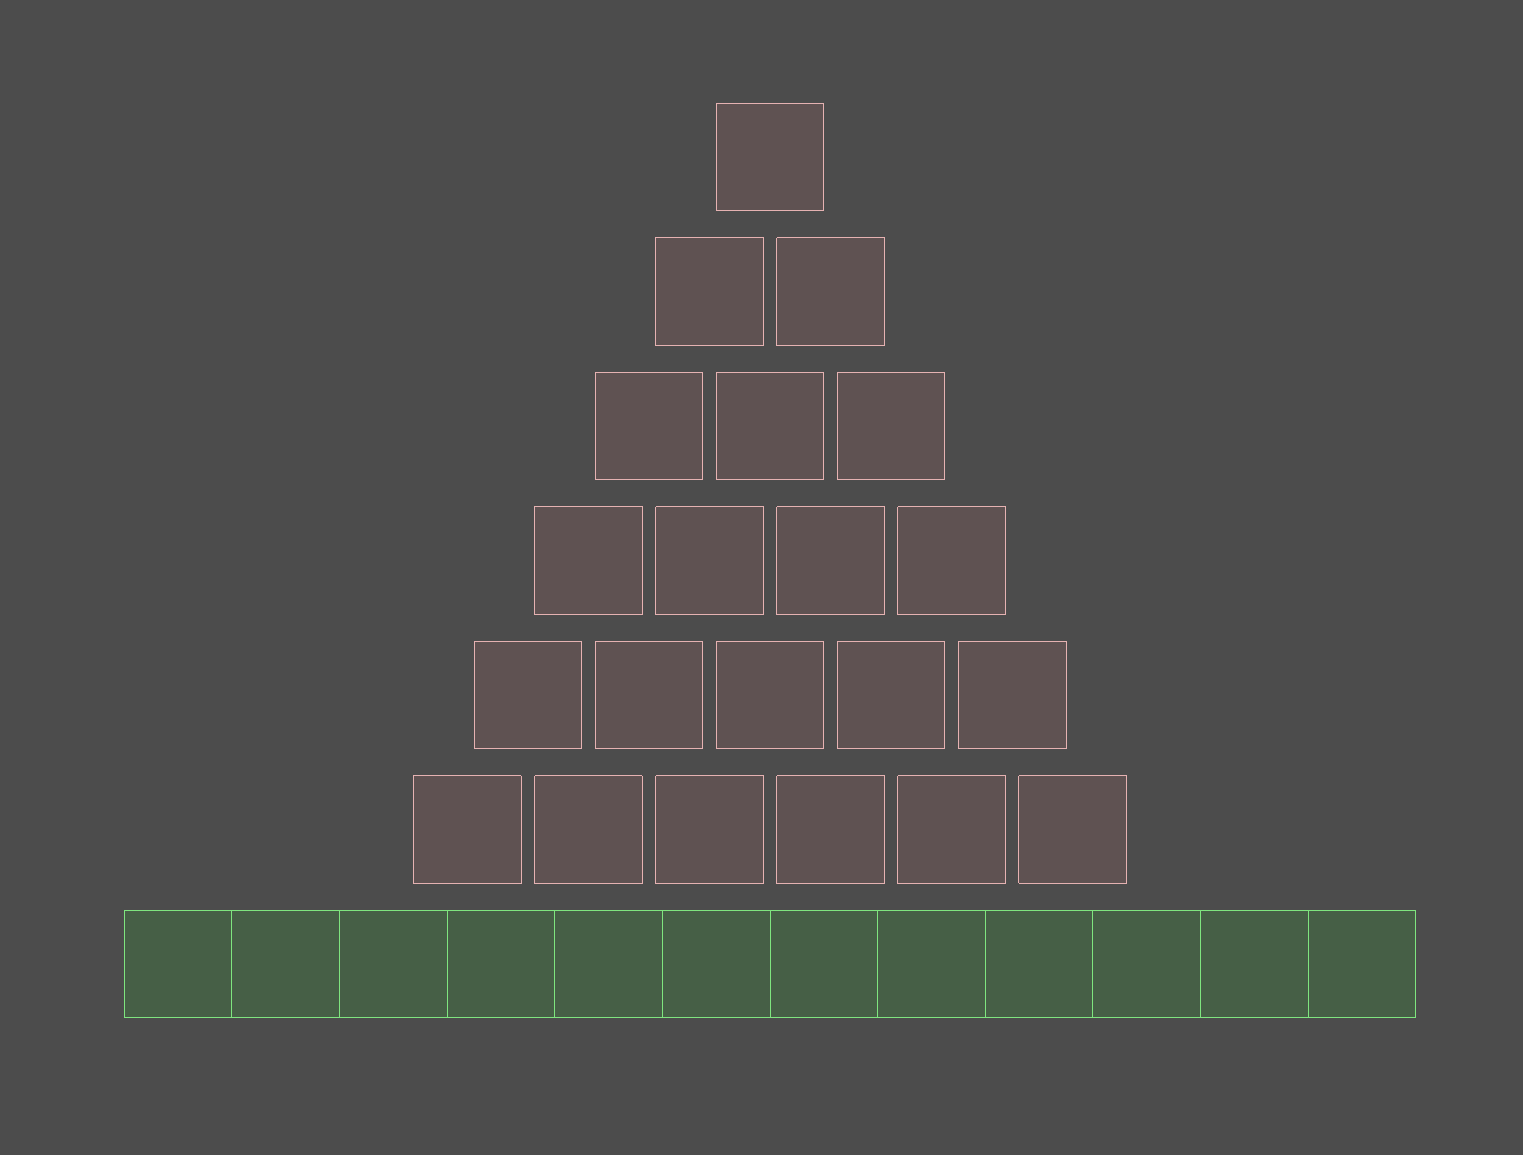
\includegraphics[width=0.5\textwidth]{Pyramid}
	\end{center}
	\caption{ Pyramid test from Box2D. Each box is 1-by-1 units (perimeter = 4).}
	\label{fig:pyramid}
\end{figure}

Figure~\ref{fig:pyramid_base} shows the resulting tree built by insertion and no rotations are used in Stage 3. Figure~\ref{fig:pyramid_rotate} shows the tree built using rotation operations in Stage 3. No height control was used. Using rotations reduces the tree height from 13 to 6 and reduces the internal node area from 391 to 317 (excluding the root node).

\begin{figure}
	\begin{center}
		\includesvg[pretex=\tiny, height=8cm]{PyramidBase}
	\end{center}
	\caption{ Pyramid test built without rotations. Leaf nodes are drawn as points and have an perimeter of 4. The total internal node area is 391 (excluding the root node). The tree height is 13. }
	\label{fig:pyramid_base}
\end{figure}

\begin{figure}
	\begin{center}
		\includesvg[pretex=\tiny, width=0.8\textwidth]{PyramidRotate}
	\end{center}
	\caption{ Pyramid test built with rotations. Leaf nodes are drawn as points and have an perimeter of 4. The total internal node area is 317 (excluding the root node). The tree height is 6. }
	\label{fig:pyramid_rotate}
\end{figure}

\section{Conclusion}

\bibliographystyle{acm}
\bibliography{DynamicTree}

\end{document}
